\documentclass{beamer}
\usepackage{enumerate}
\usepackage[utf8]{inputenc}
\usepackage{graphicx}
\usepackage{beamerthemesplit}
\usepackage{srcltx}
\usepackage{cite}
\usepackage{amsmath, amsthm, amssymb, amsfonts}
\usepackage{pgf,pgfarrows,pgfnodes,pgfautomata,pgfheaps,pgfshade,pgfpages}
\usepackage{times}
%\usepackage[normalem]{ulem}
%\usepackage{contour}

%\setbeamercovered{dynamic}%Overlay
\usecolortheme{seahorse}
%\setbeamertemplate{navigation symbols}[only frame symbol]%Навигация
\usetheme{Szeged}
\useinnertheme{rounded}
\useoutertheme{shadow}
\usefonttheme{structuresmallcapsserif}
%\beamertemplateshadingbackground{red!5}{yellow!15}
\beamertemplatenavigationsymbolsempty

%%%%%%%%%%%%%%%%%%%%%%%%%%
\newcommand{\be}{\begin{equation}}
\newcommand{\ee}{\end{equation}}
\newcommand{\scs}{\scriptstyle}

\newtheorem{mydef}{Definition}

\definecolor{gold}{rgb}{1.,0.64,0.26}
\definecolor{JungleGreen}{cmyk}{0.99,0,0.52,0}
\definecolor{BlueGreen}{cmyk}{0.85,0,0.33,0}
\definecolor{RawSienna}{cmyk}{0,0.72,1,0.45}
\definecolor{Magenta}{cmyk}{0,1,0,0}

\begin{document}

\title[PyTraceBugs: A Large Python Code Dataset for Software Defect Prediction]{PyTraceBugs: A Large Python Code Dataset
for Supervised Machine Learning
in Software Defect Prediction}
\author[E. N. Akimova et.al]{\begin{block}{}\begin{center} {E. N. Akimova, A. Yu. Bersenev, A. A. Deikov, K. S. Kobylkin,\\ A. V. Konygin, I. P. Mezentsev, V. E. Misilov} \\
{\footnotesize Krasovskii Institute of Mathematics and Mechanics,}\\
{\footnotesize Ural Federal University, Ekaterinburg, Russia}\\
{\textsl{The 28th Asia-Pacific Software Engineering Conference, \\ online, 6-9 December, 2021}}\end{center}\end{block}}
\date{}
\begin{frame}
\titlepage
\end{frame}


\section{Introduction}
%\subsection{Bugs in software}

\begin{frame}
%\frametitle{Impact of bugs on the software development}
\frametitle{Bugs in the software development}

Bugs in complex software projects have a variety of undesirable consequences,
including:
\begin{itemize}
\item data loss;
\item program crashes;
\item hardware failures.
\end{itemize}
All these issues could increase cost of software development
and lead to significant money losses. 
\newline

The task of automatically detecting bugs is a longstanding problem in the software engineering.

\end{frame}


%\begin{frame}
%\frametitle{Bugs forms}

%Finding bugs is a longstanding problem in the software engineering.
%One can distinguish between the following (possibly overlapping) forms:

%\begin{block}{Bugs forms}
%\begin{itemize}
%\item defects (e.g. when a function implementation is too complex to understand and maintain, some of possible exceptional situations/program states is not handled, etc);
%\item bugs, which lead/may lead to unexpected programs behaviours (e.g. causing them to crash);
%\item anomalies, which are not essentially bugs, but represent some unusual coding practices, not following prescribed standards.
%\end{itemize}
%\end{block}

%\end{frame}


%\begin{frame}
%\frametitle{Bugs granularities}

%Bugs can be at the following granularities:
%\begin{block}{Bugs granularity}
%\begin{itemize}
%\item module;
%\item file;
%\item class;
%\item function/method (simply, snippet);
%\item range of lines.
%\end{itemize}
%\end{block}

%\end{frame}

%\subsection{Bugs in Python}

\begin{frame}
\frametitle{Specifics of Python language}

Python is a language of choice for many developers working 
in a variety of domains, including 
web development, data science, and machine learning.

\begin{block}{Python specifics}
\begin{itemize}
\item dynamic typing;
\item its interpreter and existing static analysis tools do not
provide any thorough checks of source code.
\end{itemize}

This
postpones revealing of bugs to the runtime stage 
and leads to the need of expensive debugging stage 
during the development. 
%which might be costly.
\end{block}


\end{frame}


%\begin{frame}
%\frametitle{Specifics of Python bugs}

%\begin{alertblock}{Our aim}
%Our focus is on identifying bugs in Python functions/methods source code implementations,
%which cause programs stop working.
%\end{alertblock}


%\end{frame}


%\subsection{Deep learning methods}
\begin{frame}
\frametitle{Deep learning methods for bug prediction in Python source code}

\begin{itemize}
\item applying deep learning methodologies originally intended for natural language processing tasks (say, Transformers) to the software engineering leads to dramatic improvements;
\item using those methodologies (e.g. graph neural networks) for finding bugs in Python source code also gives promising results (Allamanis et. al, 2021).
\end{itemize}

\begin{block}{Specifics of deep learning models}
\begin{enumerate}
\item have lots of parameters;
\item require large datasets for their training.
\end{enumerate}
\end{block}

\end{frame}


\section{Related work}


\begin{frame}
\frametitle{Code analysis tasks, underlying known datasets}

Not every known bug dataset is suitable for training and evaluating deep learning models. Some of these datasets are intended for 
other tasks.% than fitting neural networks.

%\begin{block}{Possible purposes}
%\begin{enumerate}
%\item automatic test generation: tests must fail on buggy code pieces and pass on fixed pieces;
%\item program repair: learn typical patterns of fixing source code and reproduce them to automatically fix buggy code;
%\item bug prediction: report if a code piece contains bugs.
%\end{enumerate}
%\end{block}

\scriptsize{
\begin{table}
%\caption{Summary of the known datasets}
\begin{tabular}{|l|l|l|}
\hline
Task & \begin{tabular}[c]{@{}l@{}}Key Feature\\ of Dataset\end{tabular} & Description \\ \hline
Automatic Test Generation & Reproducibility & \begin{tabular}[c]{@{}l@{}}Consistent results: tests\\ should fail on buggy code \\ and pass on the fixed one.\end{tabular} \\ \hline
Program Repair & Isolation & \begin{tabular}[c]{@{}l@{}}Buggy and fixed code should\\ differ only by a bug fix.\end{tabular} \\ \hline
Bug Prediction & \begin{tabular}[c]{@{}l@{}}Representativeness\\ Sufficient size\end{tabular} & \begin{tabular}[c]{@{}l@{}}The properties of samples\\ should correspond to the\\ properties of parent classes\\ (buggy and correct code).\end{tabular} \\ \hline
\end{tabular}
\end{table}
}

\end{frame}

\begin{frame}
\frametitle{Content of the known datasets}

Tasks, underlying datasets, restrict them to contain a specific type of information.
For example, datasets aimed to either automatic test generation or program repair usually contain the so called bugfixes. 
\newline

Each bugfix contains two consequtive versions of the same source code,
where the first piece contains bugs whereas the second one is an immediate fix of those bugs.
\newline

Fixed parts of bugfix pairs can not be guaranteed to be correct. Therefore,
they do not fully represent the class of correct code.

\end{frame}


\begin{frame}
\frametitle{Summary of the known datasets}

{\tiny
\begin{table}
%\caption{Summary of the known datasets}
\begin{tabular}{|l|c|c|r|c|c|}
\hline
    Name & Language & Granularity & Size & Task & Content type \\
\hline
    ManyBugs & C & module & 185 & test generation & bugfix pairs\\
    Defects4J & Java & module & 357 & test generation & bugfix pairs\\
    Bugs.jar & Java & module & 1158 & test generation & bugfix pairs\\
    BugsInPy & Python & file & 493 & test generation & bugfix pairs\\
    GHPR & Java & file & 3026 & bug prediction & bugfix pairs\\
	BugHunter & Java & file/class/snippet\footnote{snippet means either a function or a method} & 159k & bug prediction & bugfix pairs \\
	PyPiBugs & Python & snippet & 2374 & program repair & bugfix pairs \\
    CodRep & Java & 1 line & 800k & program repair & bugfix pairs \\
    ManySStuBs4J & Java & 1 line & 153k & program repair & bugfix pairs \\
%    RANDOMBUGS\footnote{M.Allamanis et al, Self-supervised bug detection and repair, 2021} & Python & snippet & 1M & program repair & synthetic bugfix pairs \\
\hline
\end{tabular}
\end{table}}


\end{frame}

\section{PyTraceBugs dataset}
%\subsection{Features of the PyTraceBugs dataset}
\begin{frame}
\frametitle{Introducing the PyTraceBugs dataset}

{\tiny
\begin{table}
%\caption{Summary of the known datasets and our contribution}
\begin{tabular}{|l|c|c|r|c|c|}
\hline
    Name & Language & Granularity & Size & Task & Content type \\
\hline
    ManyBugs & C & module & 185 & test generation & bugfix pairs\\
    Defects4J & Java & module & 357 & test generation & bugfix pairs\\
    Bugs.jar & Java & module & 1158 & test generation & bugfix pairs\\
    BugsInPy & Python & file & 493 & test generation & bugfix pairs\\
    GHPR & Java & file & 3026 & bug prediction & bugfix pairs\\
	BugHunter & Java & file/class/snippet\footnote{snippet means either a function or a method} & 159k & bug prediction & bugfix pairs \\
	PyPiBugs & Python & snippet & 2374 & program repair & bugfix pairs \\
    CodRep & Java & 1 line & 800k & program repair & bugfix pairs \\
    ManySStuBs4J & Java & 1 line & 153k & program repair & bugfix pairs \\
%    RANDOMBUGS & Python & snippet & 1M & prog. repair & synth. bugfix pairs \\
\hline
    \textbf{PyTraceBugs} & \textbf{Python} & \textbf{snippet} &  \textbf{\begin{tabular}[c]{@{}r@{}}24k buggy\\ 5.7M correct\end{tabular}} & \textbf{bug prediction} & \textbf{\begin{tabular}[c]{@{}r@{}}buggy code\\ correct code\end{tabular}} \\
\hline
\end{tabular}
\end{table}}

%{\small
%In distinction to the known datasets, PyTraceBugs dataset is collected for the bug prediction, considered in the form of the binary classification problem with two classes of snippets:
%\begin{itemize}
%\item buggy code; 
%\item error-free (or stable) code.
%\end{itemize}}
\end{frame}

\begin{frame}
\frametitle{Purpose of the PyTraceBugs dataset}

\begin{block}{Aim of the dataset}
In distinction to the known datasets, PyTraceBugs dataset is collected specifically for pre-training and fine-tuning the deep learning models for the bug prediction problem at the granularity of snippets (implementations of functions or methods). 

This problem is considered in the form of the binary classification one with two classes of snippets:
\begin{itemize}
\item buggy code; 
\item error-free code.
\end{itemize}
\end{block}

%\begin{block}{Aim of the dataset}
%\begin{itemize}
%\item 
%PyTraceBugs is a large dataset of Python source code, containing snippets labeled either buggy or correct;
%\item 
%The dataset is aimed to pre-training and fine-tuning deep learning models for the bug prediction task.
%\end{itemize}
%\end{block}

PyTraceBugs contains a large number of Python source code snippets labeled either buggy or correct.
%It is intended for pre-training and fine-tuning deep the learning models.

\end{frame}


\begin{frame}
\frametitle{Principles, guiding labeling of snippets}

\begin{itemize}
\item PyTraceBugs contains automatically labeled source code snippets from well-maintained Github repositories for real-world software projects.
\item Buggy code is extracted by processing the bug reporting issues and corresponding bugfixing commits.
\item Error-free code is obtained from stable code. That means the code was not changed for a long time up to the current state of the repository.
\end{itemize}
\end{frame}


\begin{frame}
\frametitle{Bugs in the PyTraceBugs dataset}

\begin{block}{Specifics of bugs from the dataset}
%Bugs from the dataset manifest themselves in the form of program breaks, accompanied with
%error exception reports, containing tracebacks of functions/methods calls, causing their corresponding Python programs stop.
The dataset only includes those bugs which cause program to stop and throw an error exception report, containing the traceback information.
\end{block}

\begin{center}
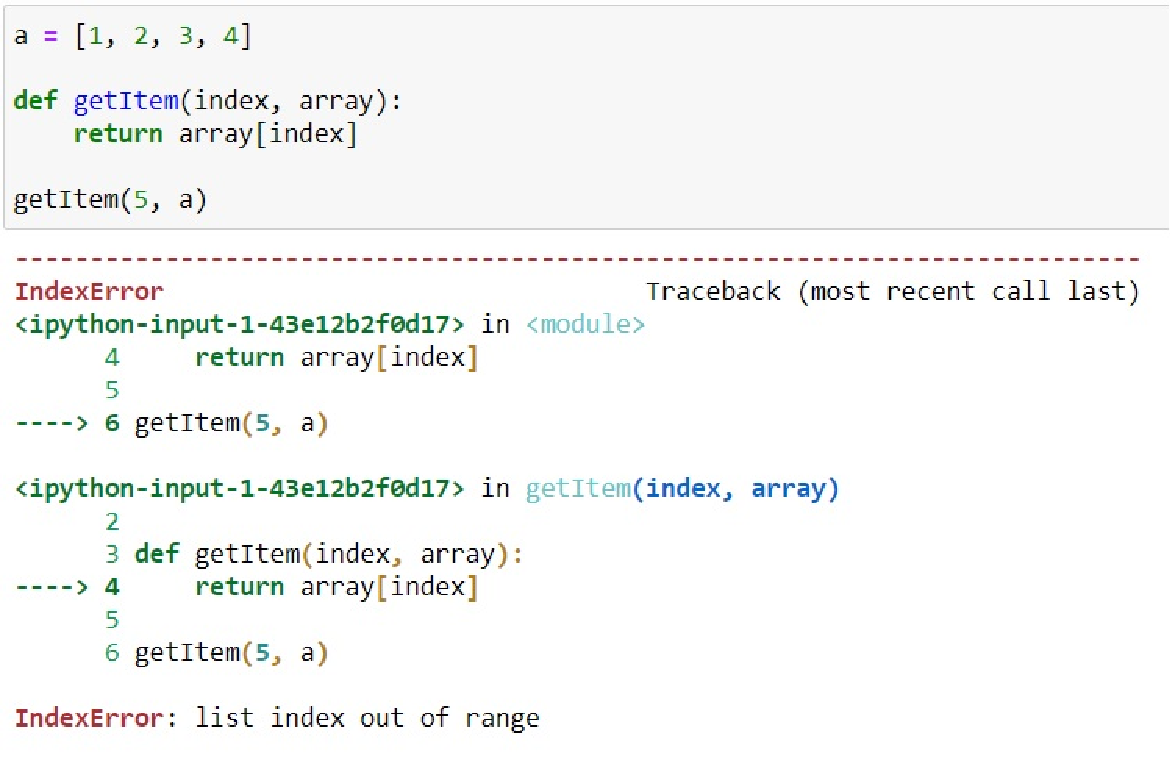
\includegraphics[height=3.5cm, width=5.6cm]{traceback.pdf}
\end{center}

The most present bugs are errors related to missing object attributes and empty objects.
\end{frame}

\begin{frame}
\frametitle{Description of the PyTraceBugs dataset}

%{\small
\begin{block}{Structure and content of the dataset}
It is split into training, validation, and test samples.
\begin{itemize}
\item training and validation samples contain automatically labeled source code snippets;
%\item buggy code from those samples is taken from bugfix pairs of snippets, extracted from bugfix commits;
%\item error-free code is obtained from stable code of repositories;
\item test sample of 330 snippets contains manually curated buggy code and selected stable code;
\item training and test samples are taken from distinct repositores.
\end{itemize}
\end{block}

%In distinction to the dataset of (Allamanis et al, 2021), both training and validation samples 
%contain real bugs, i.e. not artificially generated ones.
%}

\end{frame}


\section{Dataset quality}


\begin{frame}
\frametitle{Confidence of labeling in training and validation samples}

%To measure amount of noise in the dataset, a percentage is
%estimated of buggy snippets, for which changes, introduced in their corresponding fixed versions
%from bugfix commits and pull requests, are confined to refactoring.

To evaluate the quality of the dataset, the amount of noise (persentage of mislabeled buggy snippets) is estimated.
The mistakenly labeled buggy snippet is that for which its corresponding fix changes the test code, comments, docstrings, or is confined to code refactoring.

\begin{block}{Ways to evaluate amount of noise}
\begin{itemize}
\item the lower bound is the percentage of the changes bound to docstrings and
comments (2.6\%);
\item the percentage of refactoring changes is estimated by manually observing a random sample of several hundreds of snippets (10–15\%).
\end{itemize}
\end{block}

\end{frame}

\begin{frame}
\frametitle{Confidence of labeling in the test sample}

The test sample was validated manually by Python experts. Thus, the confidence of labeling is almost 100\%.
%Confidence of labeling of snippets in the test sample is made almost 100\%, applying manual validation
%by two Python experts.

\begin{block}{Principles guiding the manual validation}
\begin{itemize}
\item a bug reported on the web page of the corresponding
issue is simple to understand;
\item a fix of the bug introduced into a buggy snippet is also simple;
\item the reported bug is not dependency, compatibility, or the
regression bug;
\item correct snippets are chosen from stable snippets the restriction that
the snippet should be called many times from other snippets.
\end{itemize}
\end{block}


\end{frame}

\begin{frame}
\frametitle{Training predictive models on the dataset}

An alternative way to demonstrate quality of the dataset consists in
building predictive models using its data.

\begin{block}{Details of training predictive model}
\begin{itemize}
\item multi-language pretrained
CodeBERT model is applied to compute embeddings of source code from the dataset;
\item LightGBM classifier is trained on the computed embeddings.
\end{itemize}
\end{block}

\small{Results of the prediction experiments on the test sample}
{\small
\begin{table}[htbp]
%\caption{Results of the prediction experiments on the test sample}
\begin{center}
\renewcommand{\arraystretch}{1.2}
\begin{tabular}{| c | c | c | c |}
\hline
    & Precision & Recall &$F_1$-measure \\
\hline
  Correct & 0.61 & 0.99 & 0.76 \\
\hline
  Buggy & 0.96 & 0.34 & 0.5 \\
\hline
\end{tabular}
\label{tab8}
\end{center}
\end{table}}

\end{frame}

\section{Conclusion}

\begin{frame}
\frametitle{Conclusion}

{\small
%\begin{block}{Basic takeaways}
\begin{itemize}
\item PyTraceBugs is a large labeled Python source code dataset intended for both \textbf{training and evaluating of deep learning models
for software bug prediction}. 
\item It contains \textbf{24 thousands of examples of real bugs} at the granularity of
snippets.%, \textit{i.e.}, implementations of functions or methods;
\item It contains \textbf{5.7 millions} of correct code snippets.
\item The manually curated test sample consists of \textbf{330 snippets} (both buggy and correct).
\item \textbf{Confidence in labeling} of buggy snippets is 85\% for the training and validation samples, and almost 100\% for the test sample.
\item \textbf{An accurate bug prediction model} is trained on the dataset.
%it predicts bugs with precision of 0.96 and recall of 0.34 on the manually validated test sample.
\item The dataset is available at \url{https://github.com/acheshkov/pytracebugs}.
\end{itemize}
%\end{block}
}

\end{frame}

\begin{frame}

{\Large
\begin{center}
THANK YOU FOR YOUR ATTENTION!
\end{center}}



\end{frame}

\end{document}




